\documentclass{article}

\usepackage{amsmath} % operaçõess matematicas avançadas
\usepackage{graphicx} % permite imagens
\usepackage{subfigure}

\begin{document}
	\paragraph{1.}Para o produto interno não há melhoras a serem feitas logo está implementado trivialmente.
	\paragraph{2.}
		Para tentar evitar o overflow, primeiro eu procurei qual era o maior número em modulo que tem no vetor, já que, como cada um seria elevado ao quadrado, o sinal não faz diferença, e a única coisa que importa é o tamanho do número. Logo o vetor fica com essa cara: $max*\sqrt{(x_{1}/max)^2 + ... + (x_{n}/max)^2}$, evitando que numero grandes sejam elevados ao quadrado mas podendo criar números bem pequenos que ao serem elevados ao quadrado podem acabar não sendo contados na soma, que é bem difícil por estar usando o double, mas ainda assim é possível que ocorra mas não creio que iria ter grande impacto no resultado final, já que, o tamanho o erro vai se diluir no meio da soma de números muito grandes.
		Para evitar divisão por 0, fiz um 'if' tirar o caso do maior número ser 0, no caso da vetor ser nulo.
		E no teste feito somando um vetor de tamanho 1000000, onde todas as posições do vetor possuem tamanho $99999999999999999999999999999999999999.0^{4}]$ teve como resultado respectivamente 
		para o método dividindo pelo máximo e não dividindo:
		\paragraph{}9.9999987211428306E+154
		\paragraph{}Infinity
		\paragraph{}Mostrando que o método funciona.
		
	\paragraph{3.}
		Como esse EP foi feito em FORTRAN, percorri a matriz por colunas para diminuir o tempo de acesso de memoria, multiplicando o item $x_{i}$, do vetor x, por cada uma das colunas da matriz $A^{n,m}$, que aos serem todas somadas dará o vetor b.
		Os gráficos a seguir mostram a disparidade dos resultados
	\begin{figure}[h]
		\subfigure{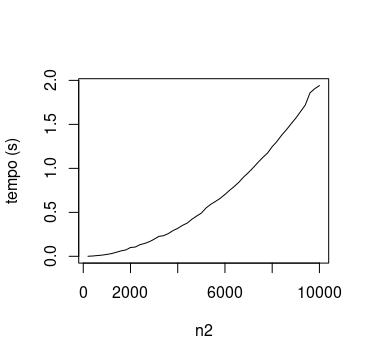
\includegraphics[width=5cm]{vet1.png}}
		\qquad
		\subfigure{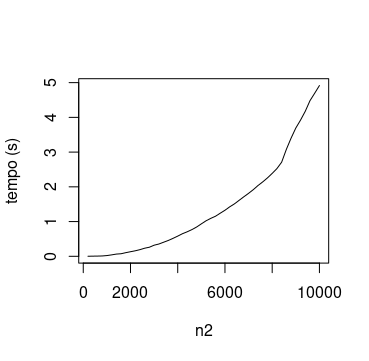
\includegraphics[width=5cm]{vet2.png}}
	\end{figure}
	
	\paragraph{}
		Tendo uma boa diferença de tempo entre os testes feitos
	
	\paragraph{4.}
		Assim como na anterior, implementei o para fazer a multiplicação de matrizes indo de coluna em coluna, ou seja, o item $a_{i,j}$ da matriz $X^{m,p}$, com i indo de 1 até p, multiplica a coluna j da matriz $A^{n,m}$ e somando o resultado com a coluna j da matriz $B^{n,p}$, que começa toda zerada.
		Ou seja, a implementação feita percorre as colunas das 3 matrizes, deixando o tempo de procura em memória mais rápida.
		Os gráficos mostram a disparidade nos tempos de execução:
		
	\begin{figure}[h]
		\subfigure{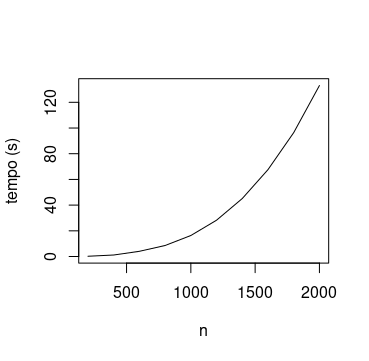
\includegraphics[width=5cm]{graf1.png}}
		\qquad
		\subfigure{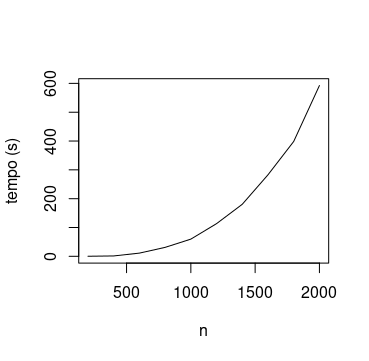
\includegraphics[width=5cm]{graf2.png}}
	\end{figure}
	
	\paragraph{}
		Sendo o primeiro o jeito feito como descrito e o segundo feito da forma trivial, sendo os tempos de execução bem diferentes.
	\paragraph{Obs.:} As funções implementadas são iguais as funções escritas como base, com exceção do tamanho da coluna das matrizes, que foram todas alocadas pelo tamanho que a matriz terá (ao invés de fixo como descrito EP)
	\paragraph{Obs.2:} Para compilatar o programa basta dar "make" e para executar "./ep1"
		
\end{document}